% Included after the main bibliography; supplementary citations use its reference keys.
\section*{Supplementary Methods and Results}
\setcounter{section}{0}
\setcounter{subsection}{0}
\setcounter{table}{0}
\setcounter{figure}{0}
\renewcommand{\thesection}{S\arabic{section}}
\renewcommand{\thetable}{S\arabic{table}}
\renewcommand{\thefigure}{S\arabic{figure}}
\renewcommand{\theHsection}{supp.\arabic{section}}
\renewcommand{\theHtable}{supp.\arabic{table}}
\renewcommand{\theHfigure}{supp.\arabic{figure}}


This supplement reports retained outputs and reproducibility details for the three-protein analysis. It does not introduce new rate estimates, model fits or structural calculations. The complete-precision tables, residue mappings, commands and selected archived outputs are supplied in \path{supplementary_data/}. Public repository deposition remains pending.

\section{Supplementary Methods}

\subsection{Structural coordinates, mappings and eligibility}

All five references have both experimental states and complete adjacent-ring shells in the stored structural QC. Canonical indices are zero-based, consecutively assigned to aligned cross-state residue pairs (gapped segments receive no index); \path{seqres_pos} is one-based extended entity sequence position. The residue-mapping CSV preserves author residue numbers in both states, canonical indices, contact counts, eligibility and descriptor values for every recorded position. Gaps and unresolved residues are not assigned coordinates. The two author chain sets are case-sensitive; operator-derived AFP copies are distinct from the deposited chain names. A selected contact-reference subunit key was not archived.

The implementation prefers non-terminal family subunits and then the candidate with the largest number of subunit centroids at strictly less than 90 \AA{}. Python \path{max} retains the first candidate in input order when scores tie. The original mmCIF bytes, selected keys, candidate scores and tie counts are absent, so exact historical subunits cannot be verified from the archived outputs. The accompanying \path{REPRODUCIBILITY_AUDIT.md} documents the ordered-input procedure and separates downstream input replay from structural reconstruction. Residue correspondence uses global BLOSUM62 alignment with opening \ensuremath{-}11 and extension \ensuremath{-}1. Modeled amino acids require C\ensuremath{\alpha}; family matching requires at least 90\% identity, calculated as the number of identical aligned pairs divided by the shorter modeled sequence length. Cross-state mismatches remain aligned when the family meets this criterion. The continuous producer does not implement an engineering mask or the earlier pilot's 8 \AA{} exclusion. Thus neither an engineering exclusion nor a specific unlogged central chain is claimed. Direct PDB chain examples in the main table identify family membership rather than the computational reference copy.

R2, SalCIS and diffocin use deposited copies; AFP applies deposited biological-assembly operators in both states. No retained reference needs guessed screw-based ring completion. The producer's generated-contact flag detects ring-completion keys, rather than all operator-derived coordinates. Its zero value must not be used to deny AFP operator expansion. Contact identity includes partner family, relative ring, relative azimuth modulo inferred ring multiplicity and canonical partner residue. Intramonomer pairs are excluded; another copy of the same family is eligible. Only matched partner positions contribute. Primary eligibility requires a contact union of at least three at strictly less than 5 \AA{}.

The archived cutoff and domain sweeps in Figure~\ref{fig:supp1} describe the structural metric only. They were not used to select a rate-association model. Changing the contact cutoff changes both eligible-site composition and mean remodeling; for example, Afp2 means range from 0.49 to 0.62 over the saved 4--6 \AA{} sweep. These records do not support blanket numerical invariance to the cutoff.

\subsection{Retrieval and positional assignment}

UniProtKB release 2026\_03, released 2 September 2026, supplied bacterial Pfam family pools. Reference UniProt identifiers are listed below. Single-query BLAST+ 2.17.0+ searches used E \ensuremath{\leq} \(10^{-5}\), \path{-seg no} and \path{-max_target_seqs 20000}. Candidate gates were 30--90\% identity, at least 80\% query coverage, and a 0.75--1.30 sequence-length ratio. The best bitscore per species was retained. These filters describe a candidate set and do not establish orthology. AFP's 5,470 joint prescreen records and 279 reference-subfamily screened members are a separate route; missing single-query funnel stages are not replaced by inferred counts.

Annotated genomic neighbourhoods extend \ensuremath{\pm}25 kb around a candidate. Flanking CDS homology was searched against the reference neighbourhood using BLAST with E \ensuremath{\leq} \(10^{-5}\), \path{-max_target_seqs 10} and \path{-seg no}. Sheath genes were excluded from anchoring evidence. Offsets are candidate CDS index minus reference slot. A locus requires at least three non-sheath anchors, at least 60\% support for its modal offset, and collinearity \ensuremath{\rho} \ensuremath{\geq} 0.8 when the collinearity statistic is defined. The retained tables include loci with undefined \ensuremath{\rho}, so this last condition is not a claim that every anchored row carries a finite statistic. Direction was normalized to the sheath orientation, and positional assignment used the modal non-sheath offset. Unanchored or ambiguous positions were left unassigned.

AFP positions 0, 1 and 2 represent Afp2, Afp3 and a third sheath-like gene. Among 42 reference-subfamily loci, 31 were anchored and 35 contained a three-gene run. Across 58 assigned genes in the comparison, 55 agreed with the sequence label. The diagnostic joint FastTree phylogeny has 145 tips, including 85 labeled tips and 60 unassigned tips; the three reference tips are included in those labeled counts. Family-wide labels do not form strictly monophyletic classes. Assignment is supported within the reference subfamily, not by a claim that the joint tree alone establishes universal positional correspondence. The final rate alignments and IQ-TREE topologies are separate from that diagnostic tree.

R2's 5,133 candidate-positive proteomes contain one detected copy in 3,341, two in 1,178, three in 432, four in 99, five in 38, and at least six in 45; the maximum is 20. These are copy counts conditional on the Pfam retrieval and must not be read as an unbiased genome-wide absence screen. Among 25 tested within-genome pairs, ten exceeded the between-genome 90th-percentile distance. The 9,180 between-genome pair distances are not independent observations. Reference-lineage assignment remained ambiguous even in the most diverse single-copy candidate set; no R2 rate regression was performed.

SalCIS's family-wide locus assessment contains 55 loci, nine anchored; 28 contain two sheath-like genes and 27 one. The restricted enterobacterial assessment has 29 loci, nine anchored, with 19 single-, three double- and seven triple-sheath loci. Neither route yields an adequate corresponding reference-position sample. Diffocin has 142 loci with one local sheath gene each, 67 anchored, and 36 exact-offset assignments. Seven of 137 replicons nevertheless contain two candidate loci. Removing both ambiguous \emph{P. hiranonis} assignments gives the primary 33-sequence dataset, distinct from screened 35 and collinear-frame 66 sequence sets.

\subsection{Alignments, trees and rate-estimation settings}

FAMSA through pyfamsa 0.7.0 produced the saved alignments. A separate embedded FAMSA build version was not recorded. No final column trimming is documented. A reference-row gap is skipped when mapping alignment columns to one-based SEQRES positions. Site occupancy is the fraction of rows with a non-gap amino acid. The primary threshold is 80\%; the saved 50\% checks add only one Afp3 site. Invariant columns are retained in primary fits and excluded only in the recorded variable-site checks.

IQ-TREE 3.1.4 used ModelFinder BIC selection, 1,000 ultrafast bootstrap replicates, 1,000 SH-aLRT replicates and four threads. Exact commands and logged random seeds are in \path{archived_commands.txt}. Both AFP topologies selected WAG+I+G4; primary diffocin selected LG+F+I+G4, and both alternative diffocin sets selected Q.PFAM+F+G4. Earlier FastTree 2.2.0 LG+\ensuremath{\Gamma} phylogenies serve orthology/feasibility QC; their summary distances are not substituted for the final IQ-TREE fit.

Rate4Site self-reports version 2.01 although its ConSurf source-directory label is 3.2. The retained build patched three pre-C++11 stream idioms in error and file-open handling, without changes to numerical routines: address comparison in \path{errorMsg.cpp} and \path{!stream.is_open()} checks in \path{someUtil.cpp} and \path{rate4siteOptions.cpp}. Source/build provenance is recorded in \path{FROZEN_ANALYSIS.md}; the build source is retained in the project, not fully reproduced in this compact manuscript bundle. All runs used \path{-Mw -ib -k 16}, a fixed supplied topology (\path{-t}), and reference row \path{-a REF}. Rate4Site reoptimized branch lengths under WAG+\ensuremath{\Gamma}. It implements neither LG nor Q.PFAM, so matrix differences from the selected diffocin topology models are retained and disclosed. The saved IQ-TREE branch lengths remain in the original \path{.treefile} outputs.

Increasing normalized Rate4Site scores mean faster relative evolution. The output also retains unnormalized posterior rates and uncertainty. Invariant sites receive empirical Bayes estimates rather than a single assigned floor. The JSON field \path{invariant_sites_in_fit} counts sites with zero posterior SD, rather than alignment invariance, and is zero in the primary models. The actual invariant counts are 33, 17 and eight for fitted Afp2, Afp3 and diffocin sites. Table~\ref{tab:supp3} checks distinct non-gap amino acids in the saved alignments at the fitted reference positions. The \path{n_aa} field reports occupancy counts, not amino-acid diversity.

\subsection{Structural covariates and statistical implementation}

Shrake--Rupley uses the Biopython defaults (1.4 \AA{} probe radius and 100 surface points per atom) on an isolated chain; residue ASA is divided by Tien theoretical maximum ASA. WCN sums inverse squared C\ensuremath{\alpha} distances to all other modeled residues in that chain, including sequence neighbours. Self-pairs and squared distances \ensuremath{\leq} \(10^{-6}\) \AA{}\ensuremath{^2} are excluded. GNM uses an adjacency of 0 < d < 7.3 \AA{}, the corresponding Kirchhoff Laplacian and the diagonal of its numerical pseudoinverse. No physical fluctuation scale is inferred. Covariates use the representative chain selected during family matching, rather than the interior subunit selected for assembly contacts. The representative monomer-chain keys were not exported. The producer computes both states and writes the available-state arithmetic mean of descriptor values; it does not average atomic coordinates. Only the averaged \path{rsa}, \path{wcn} and \path{gnm} columns are retained; state-specific intermediate values cannot be checked from the tables. This differs from the written extended-state specification. The manuscript uses the archived inputs and does not choose states or refit.

For each protein, the outcome and four predictors are standardized with sample SD (\path{ddof=1}). OLS includes an intercept and uses the full available eligible sites at the specified occupancy. The partial \(R^2\) compares the full model with RSA/WCN/GNM alone. Saved standard errors, OLS intervals and p-values assume independent sites; scientific interpretation instead emphasizes the sequence-block intervals. The intercept estimate and its SE were not exported. It is centered by construction, but no unarchived intercept inferential statistic is invented in Table~\ref{tab:supp4}.

The bootstrap seed is 20261013. Block identifiers are \path{(seqres_pos - 1) // 10}. Only nonempty windows enter the draw pool; a sampled block contributes its eligible rows, so its row count need not equal ten. Blocks are repeatedly drawn with replacement until the original site count is met or exceeded; the last sampled block is truncated to that count. All variables are re-standardized in each replicate and the coefficient is estimated by least squares. The retained runs used all 10,000 replicates. Percentiles 2.5 and 97.5 yield the intervals. This scheme retains some local sequence dependence, not necessarily dependence between sequence-distant spatial neighbours. Neither full coverage under spatial dependence nor uncertainty from structures, sequence selection, phylogenies or rate posteriors is estimated by this resampling procedure.

The written variable-site sensitivity clause explicitly names Afp2. Parallel Afp3 and diffocin restrictions are present in saved results but not expressly named in that clause. Their timing relative to the clause is not recoverable from the retained record, and they are identified as archived parallel checks. The alternative diffocin sets and 50\% occupancy checks are named in the written plan. No additional regression diagnostics, measurement-error models or between-system effect tests were introduced during writing.

\section{Supplementary Results and Tables}

\subsection{Structural references and residue eligibility}

\begingroup
\footnotesize
\setlength{\tabcolsep}{3pt}
\renewcommand{\arraystretch}{1.2}
\begin{longtable}{>{\raggedright\arraybackslash}p{\dimexpr 0.19\linewidth-2\tabcolsep\relax}>{\raggedright\arraybackslash}p{\dimexpr 0.25\linewidth-2\tabcolsep\relax}>{\raggedright\arraybackslash}p{\dimexpr 0.15\linewidth-2\tabcolsep\relax}>{\raggedright\arraybackslash}p{\dimexpr 0.13\linewidth-2\tabcolsep\relax}>{\raggedright\arraybackslash}p{\dimexpr 0.13\linewidth-2\tabcolsep\relax}>{\raggedright\arraybackslash}p{\dimexpr 0.15\linewidth-2\tabcolsep\relax}}
\caption{Structural references, cross-state modeled sequences and eligibility. E/C denotes extended/contracted; copy counts include both AFP families where deposited operators are applied. Full author chain sets and residue mappings accompany the table.}\label{tab:supp1}\\
\toprule
\textbf{Protein} & \textbf{PDB/entity E/C} & \textbf{Modeled E/C} & \textbf{Identity} & \textbf{Eligible} & \textbf{Copies E/C} \\
\midrule
\endfirsthead
\multicolumn{6}{l}{\tablename~\thetable{} (continued)}\\
\toprule
\textbf{Protein} & \textbf{PDB/entity E/C} & \textbf{Modeled E/C} & \textbf{Identity} & \textbf{Eligible} & \textbf{Copies E/C} \\
\midrule
\endhead
\bottomrule
\endfoot
R2 pyocin & 3J9Q/1 / 3J9R/1 & 385/383 & 1.000 & 143 & 24/36 \\
AFP Afp2 & 6RBN/2 / 6RC8/1 & 350/348 & 1.000 & 84 & 24/48 \\
AFP Afp3 & 6RBN/3 / 6RC8/2 & 358/355 & 0.992 & 82 & 24/48 \\
SalCIS & 9R9H/1 / 9R9I/1 & 514/495 & 0.994 & 68 & 18/18 \\
Diffocin & 8V3X/1 / 8V3Y/1 & 352/353 & 1.000 & 58 & 18/30 \\
\end{longtable}
\endgroup

\textbf{R2 pyocin:} author chains E: A--R, X, a, d, g, j, m; C: 0--5, A--R, a--l. Eligible reference-position range 2--383 (not every intervening position is eligible). Coordinates: deposited copies.

\textbf{AFP Afp2:} author chains E: C; C: A. Eligible reference-position range 5--351 (not every intervening position is eligible). Coordinates: deposited operators.

\textbf{AFP Afp3:} author chains E: D; C: B. Eligible reference-position range 4--447 (not every intervening position is eligible). Coordinates: deposited operators.

\textbf{SalCIS:} author chains E: T--Z, a--k; C: O--Z, a--f. Eligible reference-position range 12--515 (not every intervening position is eligible). Coordinates: deposited copies.

\textbf{Diffocin:} author chains E: E, F, P, Q, S--X, d, e, g, n, q--s, z; C: A--Z, a--d. Eligible reference-position range 3--354 (not every intervening position is eligible). Coordinates: deposited copies.

Full mappings and deposited author chain lists are in the Table~\ref{tab:supp1} CSVs. Selected interior keys are not archived; all five reported shells are complete and no ring completion was required. Paired identities are rounded in the stored outputs.

\subsection{Retrieval counts and orthology decisions}

\begingroup
\footnotesize
\setlength{\tabcolsep}{3pt}
\renewcommand{\arraystretch}{1.2}
\begin{longtable}{>{\raggedright\arraybackslash}p{\dimexpr 0.16\linewidth-2\tabcolsep\relax}>{\raggedright\arraybackslash}p{\dimexpr 0.08\linewidth-2\tabcolsep\relax}>{\raggedright\arraybackslash}p{\dimexpr 0.15\linewidth-2\tabcolsep\relax}>{\raggedright\arraybackslash}p{\dimexpr 0.13\linewidth-2\tabcolsep\relax}>{\raggedright\arraybackslash}p{\dimexpr 0.12\linewidth-2\tabcolsep\relax}>{\raggedright\arraybackslash}p{\dimexpr 0.36\linewidth-2\tabcolsep\relax}}
\caption{Retrieval funnels and orthology decisions. AFP uses a joint prescreen rather than a directly comparable single-query gated funnel. Counts are screening-stage observations.}\label{tab:supp2}\\
\toprule
\textbf{Route} & \textbf{Pool} & \textbf{BLAST/prescreen} & \textbf{Gated} & \textbf{Species} & \textbf{Decision} \\
\midrule
\endfirsthead
\multicolumn{6}{l}{\tablename~\thetable{} (continued)}\\
\toprule
\textbf{Route} & \textbf{Pool} & \textbf{BLAST/prescreen} & \textbf{Gated} & \textbf{Species} & \textbf{Decision} \\
\midrule
\endhead
\bottomrule
\endfoot
R2 pyocin & 8035 & 4593 & 1266 & 967 & excluded: reference lineage ambiguous \\
SalCIS & 7592 & 4490 & 805 & 667 & excluded: reference locus poorly recovered \\
Diffocin & 8005 & 930 & 192 & 165 & retained: primary 33 sequences \\
AFP joint route & 8005 & 5470 & not comparable & not comparable & retained: Afp2 27 / Afp3 31 \\
\end{longtable}
\endgroup

Reference sequence identifiers: r2pyocin: Q9S574 (386 aa), Pfam PF04984, PF17482, PF22671; afp\_Afp2: Q6HAD7 (354 aa), Pfam PF04984, PF17482; afp\_Afp3: Q6HAD6 (451 aa), Pfam PF04984, PF17482; salcis: A0A701XPN5 (519 aa), Pfam PF17482; diffocin: A0A9Q7ZU73 (354 aa), Pfam PF04984, PF17482.

Counts describe recorded screening stages rather than final interchangeable ortholog sets. The AFP prescreen differs from the three single-query routes. Family-wide AFP diagnosis and reference-subfamily selection are separate. Detailed locus records are retained in the project; Figures S2--S4 summarize selected archived evidence.

\subsection{Final alignment occupancy and variability}

\begingroup
\footnotesize
\setlength{\tabcolsep}{3pt}
\renewcommand{\arraystretch}{1.2}
\begin{longtable}{>{\raggedright\arraybackslash}p{\dimexpr 0.26\linewidth-2\tabcolsep\relax}>{\raggedright\arraybackslash}p{\dimexpr 0.13\linewidth-2\tabcolsep\relax}>{\raggedright\arraybackslash}p{\dimexpr 0.14\linewidth-2\tabcolsep\relax}>{\raggedright\arraybackslash}p{\dimexpr 0.16\linewidth-2\tabcolsep\relax}>{\raggedright\arraybackslash}p{\dimexpr 0.12\linewidth-2\tabcolsep\relax}>{\raggedright\arraybackslash}p{\dimexpr 0.19\linewidth-2\tabcolsep\relax}}
\caption{Alignment metadata, fitted-site occupancy and variability. Values come from saved alignments and site tables; the alternate diffocin sets are sensitivity datasets.}\label{tab:supp3}\\
\toprule
\textbf{Dataset} & \textbf{Sequences} & \textbf{Columns} & \textbf{Fitted sites} & \textbf{Variable} & \textbf{Minimum occupancy} \\
\midrule
\endfirsthead
\multicolumn{6}{l}{\tablename~\thetable{} (continued)}\\
\toprule
\textbf{Dataset} & \textbf{Sequences} & \textbf{Columns} & \textbf{Fitted sites} & \textbf{Variable} & \textbf{Minimum occupancy} \\
\midrule
\endhead
\bottomrule
\endfoot
AFP Afp2 & 27 & 415 & 84 & 51 & 1.000 \\
AFP Afp3 & 31 & 708 & 81 & 64 & 0.903 \\
Diffocin & 33 & 515 & 58 & 50 & 0.970 \\
diffocin asscreened & 35 & 535 & 58 & 50 & 0.971 \\
diffocin collinear & 66 & 565 & 58 & 53 & 0.985 \\
\end{longtable}
\endgroup

Fitted-site counts use the retained primary or alternative site tables. Afp3 has 82 structural sites, of which one has 0.742 occupancy and is excluded at 80\%. Its 81-site primary model has 64 variable sites; the 82-site occupancy sensitivity has 65. All Afp2 structural sites have full occupancy. Primary diffocin structural sites have minimum occupancy 0.970. The supplied CSV records exact alignment paths and reference lengths.

Taxonomic breadth (effective genera) is 5.49 for Afp2, 5.43 for Afp3, 16.71 for primary diffocin, 17.71 for screened diffocin and 31.27 for collinear diffocin. AFP spans eight genera; the largest genus contributes 33.3\% and 32.3\%, respectively. Primary diffocin contains 29 species in 20 genera and its largest genus contributes 12.5\%. These are sampling summaries, not numbers of independent evolutionary replicates.

Earlier AFP feasibility trees have total lengths 6.62 and 17.02 substitutions per site, mean patristic distances 0.914 and 1.937, and maximum distances 1.683 and 5.550. The historical screened 35-sequence diffocin tree has total length 16.18, mean distance 1.592 and maximum 2.444. These QC summaries are not final IQ-TREE summaries and the 35-sequence values must not be relabeled as properties of the 33-sequence primary tree. The retained R2 best single-copy set had 136 sequences, 143 sites, eight invariant sites, effective genera 22.25 and a maximum QC patristic distance of 4.207, but was excluded on orthology rather than diversity grounds. No corresponding SalCIS rate dataset was constructed.

\subsection{Full exported primary regression coefficients}

\begingroup
\footnotesize
\setlength{\tabcolsep}{3pt}
\renewcommand{\arraystretch}{1.2}
\begin{longtable}{>{\raggedright\arraybackslash}p{\dimexpr 0.16\linewidth-2\tabcolsep\relax}>{\raggedright\arraybackslash}p{\dimexpr 0.1\linewidth-2\tabcolsep\relax}>{\raggedright\arraybackslash}p{\dimexpr 0.1\linewidth-2\tabcolsep\relax}>{\raggedright\arraybackslash}p{\dimexpr 0.1\linewidth-2\tabcolsep\relax}>{\raggedright\arraybackslash}p{\dimexpr 0.23\linewidth-2\tabcolsep\relax}>{\raggedright\arraybackslash}p{\dimexpr 0.1\linewidth-2\tabcolsep\relax}>{\raggedright\arraybackslash}p{\dimexpr 0.11\linewidth-2\tabcolsep\relax}}
\caption{All exported non-intercept primary coefficients, independent-site OLS standard errors, intervals and p-values, and variance inflation factors. Intercept inferential statistics were not exported.}\label{tab:supp4}\\
\toprule
\textbf{Protein} & \textbf{Predictor} & \textbf{\ensuremath{\beta}} & \textbf{SE} & \textbf{OLS 95\% CI} & \textbf{OLS p} & \textbf{VIF} \\
\midrule
\endfirsthead
\multicolumn{7}{l}{\tablename~\thetable{} (continued)}\\
\toprule
\textbf{Protein} & \textbf{Predictor} & \textbf{\ensuremath{\beta}} & \textbf{SE} & \textbf{OLS 95\% CI} & \textbf{OLS p} & \textbf{VIF} \\
\midrule
\endhead
\bottomrule
\endfoot
AFP Afp2 & R & +0.4351 & 0.1176 & [+0.2010, +0.6692] & 0.0003978 & 1.412 \\
AFP Afp2 & rsa & +0.2114 & 0.1420 & [-0.0712, +0.4939] & 0.1404 & 2.056 \\
AFP Afp2 & wcn & +0.2654 & 0.2212 & [-0.1749, +0.7057] & 0.2338 & 4.994 \\
AFP Afp2 & gnm & +0.1367 & 0.2089 & [-0.2790, +0.5525] & 0.5147 & 4.452 \\
AFP Afp3 & R & +0.4247 & 0.1136 & [+0.1983, +0.6510] & 0.0003582 & 1.241 \\
AFP Afp3 & rsa & +0.1947 & 0.1487 & [-0.1014, +0.4908] & 0.1942 & 2.123 \\
AFP Afp3 & wcn & +0.3290 & 0.2209 & [-0.1109, +0.7688] & 0.1405 & 4.687 \\
AFP Afp3 & gnm & +0.2791 & 0.2028 & [-0.1248, +0.6831] & 0.1728 & 3.952 \\
Diffocin & R & +0.0347 & 0.1354 & [-0.2369, +0.3063] & 0.7988 & 1.105 \\
Diffocin & rsa & +0.1341 & 0.2294 & [-0.3260, +0.5942] & 0.5612 & 3.172 \\
Diffocin & wcn & -0.5623 & 0.3731 & [-1.3107, +0.1862] & 0.1378 & 8.392 \\
Diffocin & gnm & -0.5451 & 0.2896 & [-1.1261, +0.0358] & 0.06531 & 5.056 \\
\end{longtable}
\endgroup

All four non-intercept coefficients are standardized within protein. Independent-site OLS statistics are descriptive; primary remodeling inference uses the block-bootstrap intervals in main Table~\ref{tab:primary}. Intercept inferential statistics were not archived. VIFs indicate appreciable collinearity among conventional descriptors despite relatively low VIF for remodeling. Full-precision values are preserved in the supplied CSV and original JSON.

\subsection{Complete archived sensitivity results}

\clearpage
\begin{landscape}
\begingroup
\footnotesize
\setlength{\tabcolsep}{3pt}
\renewcommand{\arraystretch}{1.2}
\begin{longtable}{>{\raggedright\arraybackslash}p{\dimexpr 0.22\linewidth-2\tabcolsep\relax}>{\raggedright\arraybackslash}p{\dimexpr 0.09\linewidth-2\tabcolsep\relax}>{\raggedright\arraybackslash}p{\dimexpr 0.07\linewidth-2\tabcolsep\relax}>{\raggedright\arraybackslash}p{\dimexpr 0.08\linewidth-2\tabcolsep\relax}>{\raggedright\arraybackslash}p{\dimexpr 0.07\linewidth-2\tabcolsep\relax}>{\raggedright\arraybackslash}p{\dimexpr 0.09\linewidth-2\tabcolsep\relax}>{\raggedright\arraybackslash}p{\dimexpr 0.18\linewidth-2\tabcolsep\relax}>{\raggedright\arraybackslash}p{\dimexpr 0.1\linewidth-2\tabcolsep\relax}>{\raggedright\arraybackslash}p{\dimexpr 0.1\linewidth-2\tabcolsep\relax}}
\caption{Complete archived sensitivity results. An asterisk marks Afp3 and diffocin variable-site checks beyond the literal Afp2-only written clause. Other specifications are named in the written sensitivity plan. Bootstrap intervals follow the primary sequence-window scheme.}\label{tab:supp5}\\
\toprule
\textbf{Specification} & \textbf{Sequences} & \textbf{Sites} & \textbf{\(\beta_R\)} & \textbf{SE} & \textbf{OLS p} & \textbf{Sequence-block 95\% CI} & \textbf{Partial \(R^2\)} & \textbf{Full \(R^2\)} \\
\midrule
\endfirsthead
\multicolumn{9}{l}{\tablename~\thetable{} (continued)}\\
\toprule
\textbf{Specification} & \textbf{Sequences} & \textbf{Sites} & \textbf{\(\beta_R\)} & \textbf{SE} & \textbf{OLS p} & \textbf{Sequence-block 95\% CI} & \textbf{Partial \(R^2\)} & \textbf{Full \(R^2\)} \\
\midrule
\endhead
\bottomrule
\endfoot
Diffocin screened & 35 & 58 & +0.0707 & 0.1358 & 0.6048 & [-0.1516, +0.3016] & 0.0051 & 0.1157 \\
Diffocin collinear & 66 & 58 & +0.1208 & 0.1372 & 0.3827 & [-0.1183, +0.3610] & 0.0144 & 0.0977 \\
Afp2 variable & 27 & 51 & +0.2748 & 0.1712 & 0.1153 & [-0.0228, +0.5446] & 0.0531 & 0.1981 \\
Afp3 variable* & 31 & 64 & +0.3550 & 0.1526 & 0.02344 & [+0.1893, +0.4902] & 0.0840 & 0.1691 \\
Diffocin variable* & 33 & 50 & -0.0589 & 0.1475 & 0.6916 & [-0.3390, +0.2338] & 0.0035 & 0.1196 \\
Diffocin occupancy 50\% & 33 & 58 & +0.0347 & 0.1354 & 0.7988 & [-0.1734, +0.2441] & 0.0012 & 0.1207 \\
Afp2 occupancy 50\% & 27 & 84 & +0.4351 & 0.1176 & 0.0003978 & [+0.2286, +0.6360] & 0.1476 & 0.2258 \\
Afp3 occupancy 50\% & 31 & 82 & +0.4190 & 0.1122 & 0.0003567 & [+0.2773, +0.5411] & 0.1535 & 0.2123 \\
\end{longtable}
\endgroup
\end{landscape}

An asterisk identifies parallel variable-site checks beyond the literal Afp2-only clause. The other rows correspond to named sensitivity specifications. These results are unchanged from the saved JSON; rounded CSVs are not used as the authoritative coefficient source. Each model retains all three structural covariates and the same sequence-window bootstrap. No association is detected in diffocin in these specifications. Afp2's variable-site interval includes zero, whereas Afp3's parallel restriction retains a positive interval.

\clearpage

\section*{Supplementary Figures}

\begin{figure}[p]
\centering
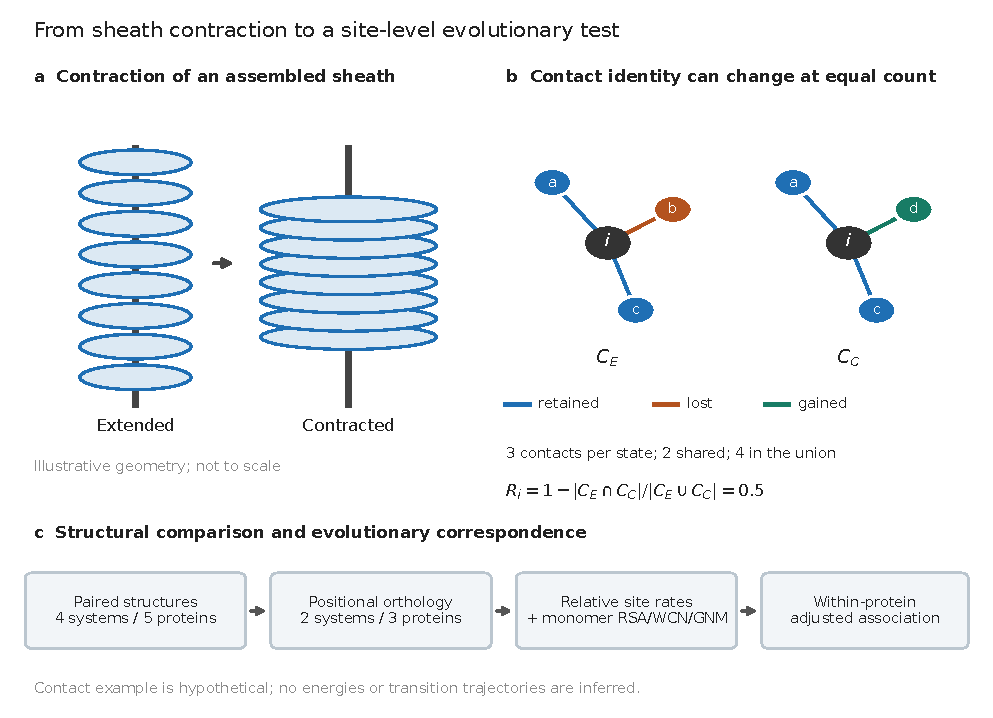
\includegraphics[width=\textwidth,height=0.34\textheight,keepaspectratio]{figures/FigureS1a.pdf}\par\smallskip
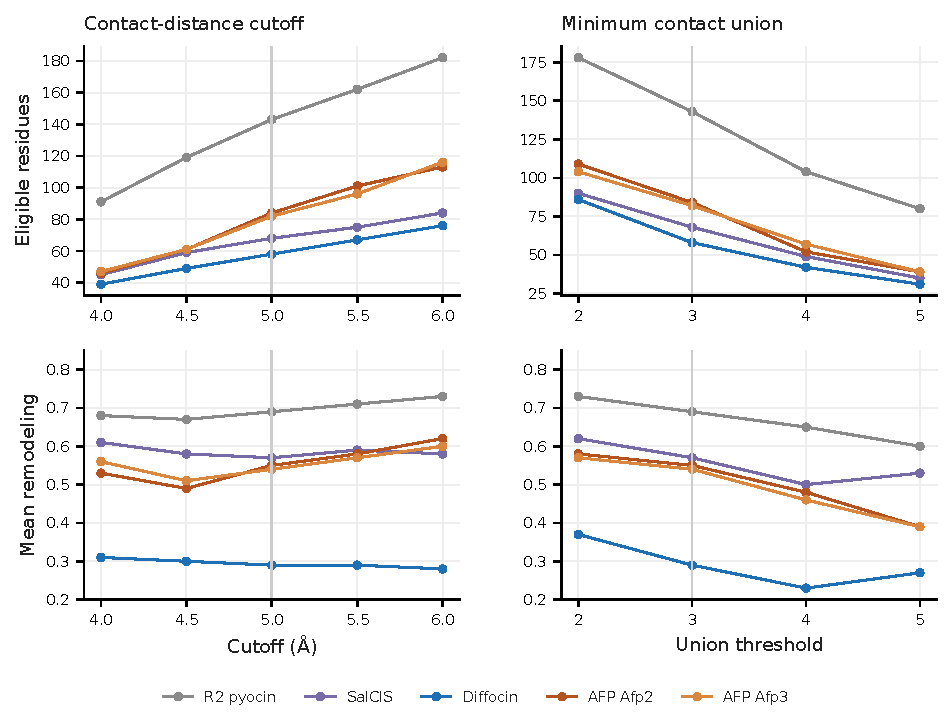
\includegraphics[width=\textwidth,height=0.37\textheight,keepaspectratio]{figures/FigureS1b.pdf}\par\smallskip
\caption{Contact-definition and mapping QC. (a) Explanatory sheath/contact-set schematic; the geometry and contact example are hypothetical and do not represent an atomic rendering. (b) Stored cutoff and union-domain sweeps show eligible-site counts and mean remodeling for the five retained references. These are structural QC summaries from the saved report, not new calculations or evolutionary sensitivity fits.}
\label{fig:supp1}
\end{figure}

\begin{figure}[p]
\centering
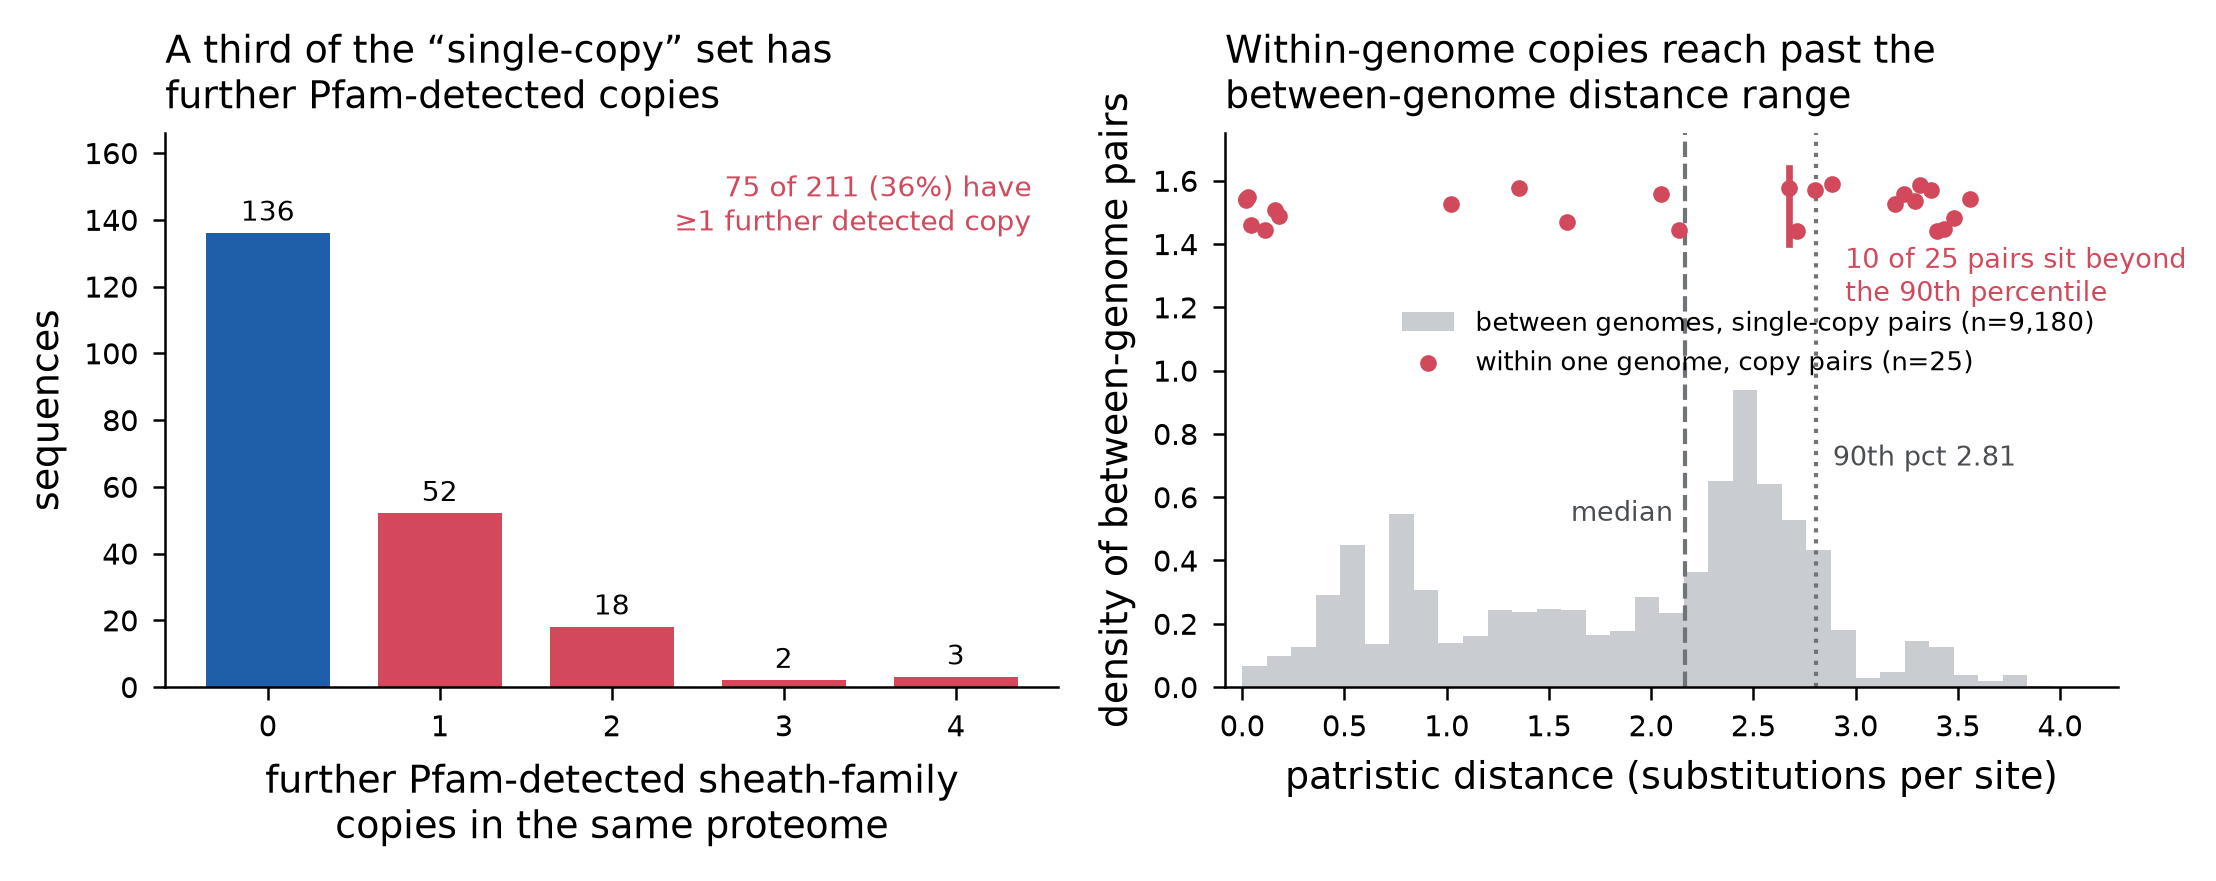
\includegraphics[width=\textwidth,height=0.30\textheight,keepaspectratio]{figures/FigureS2a.png}\par\smallskip
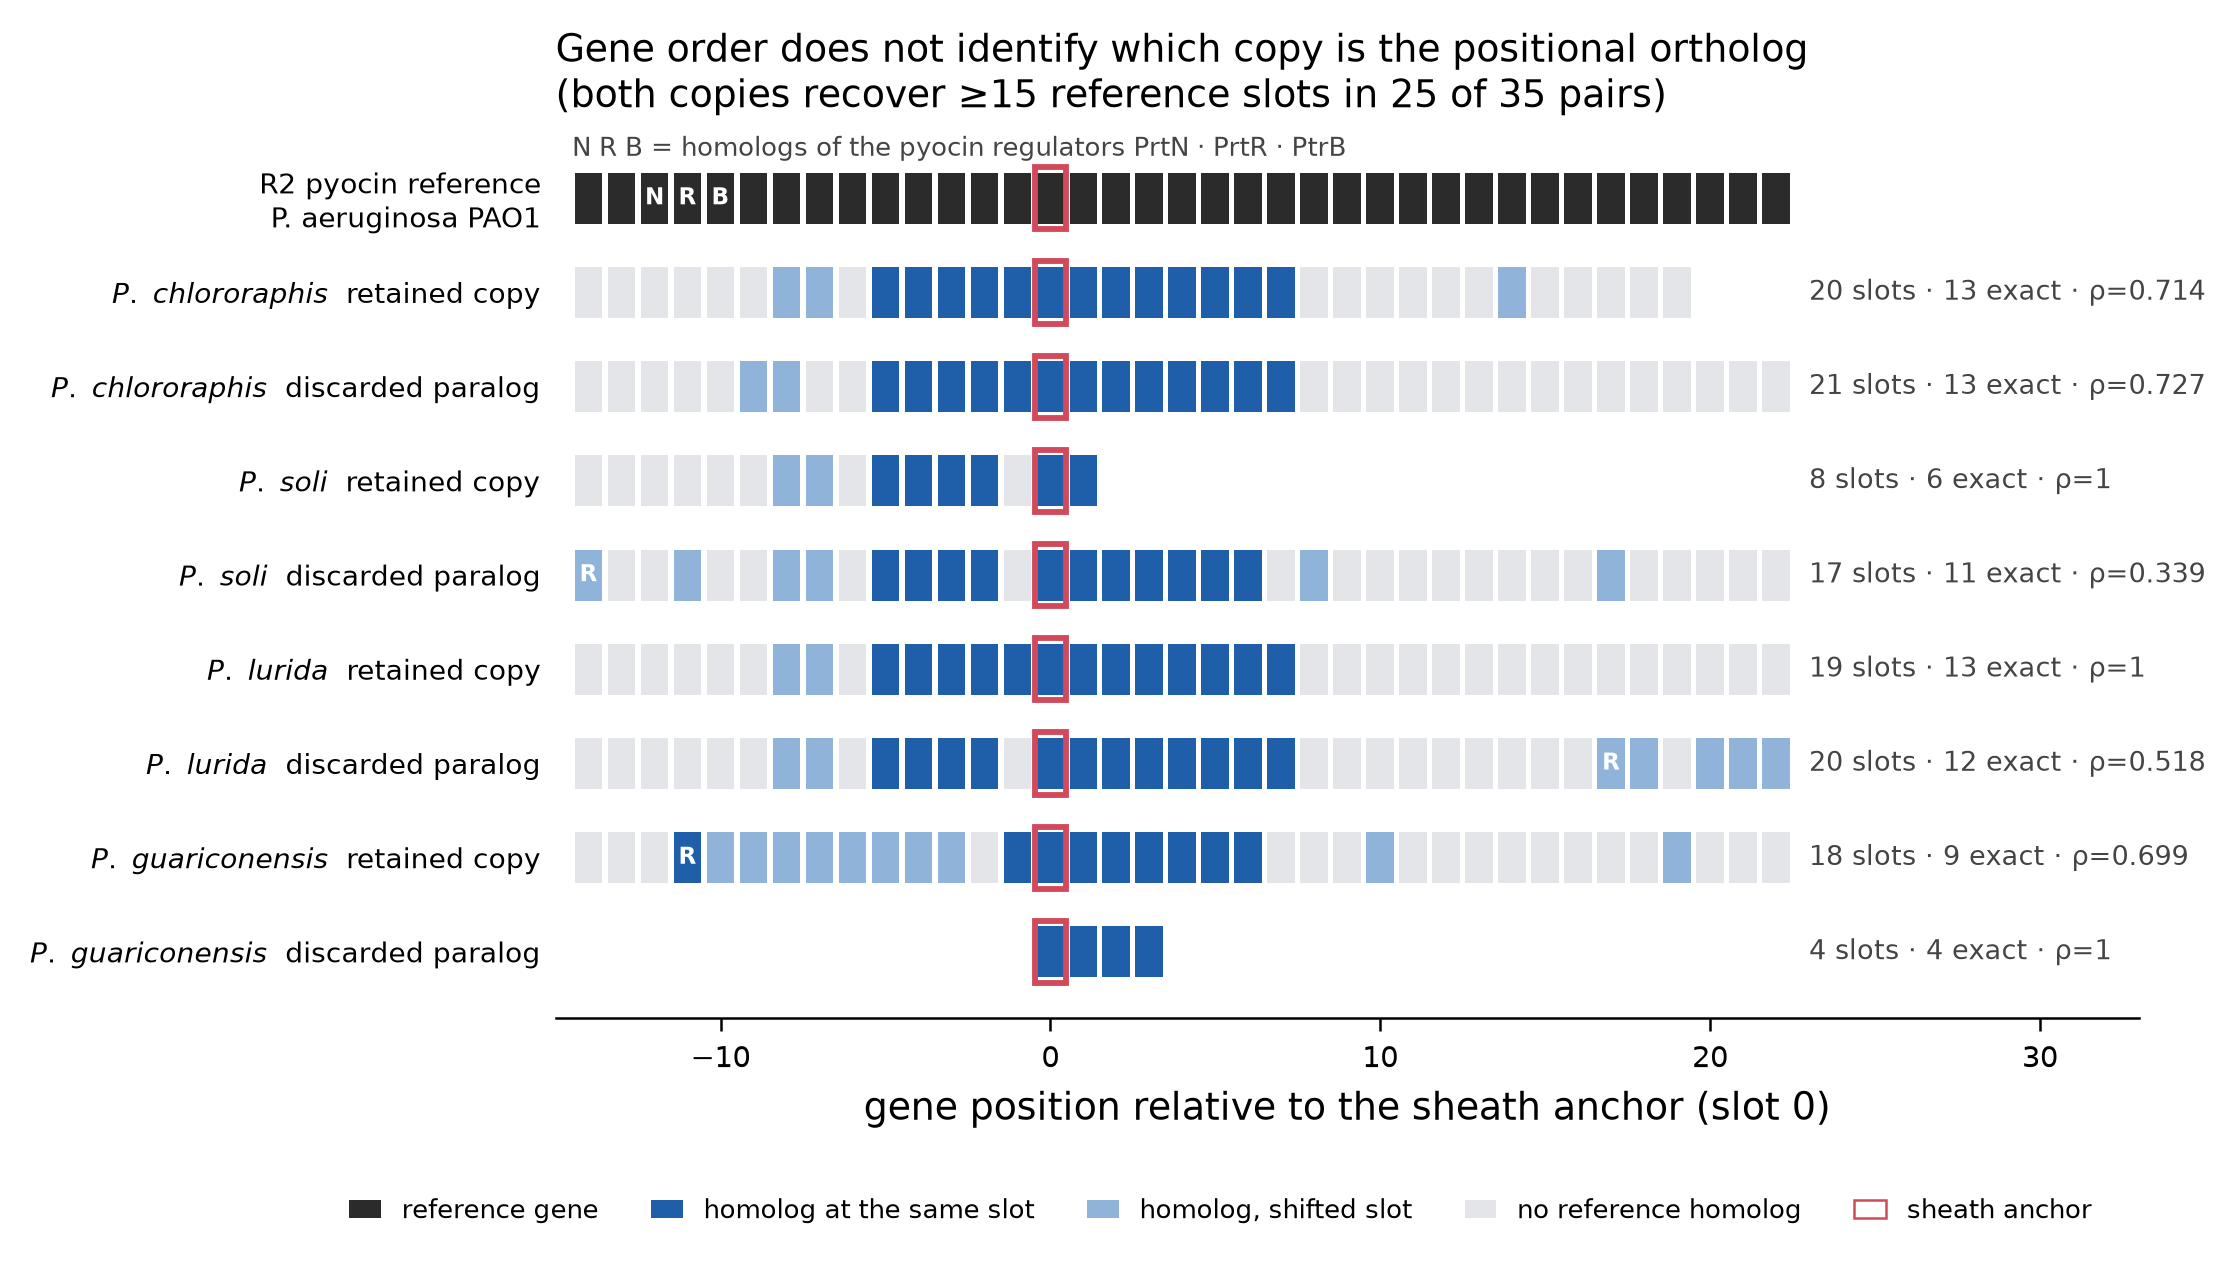
\includegraphics[width=\textwidth,height=0.38\textheight,keepaspectratio]{figures/FigureS2b.png}\par\smallskip
\caption{R2 copy-number and paralogy evidence. (a) The existing copy-number audit and within- versus between-genome distance comparison. Counts are conditional on retrieval; pair distances share sequences and are not independent. (b) Existing retained/discarded candidate locus examples illustrate reference-order ambiguity. These diagnostic candidate sets were not used for a primary rate regression.}
\label{fig:supp2}
\end{figure}

\begin{figure}[p]
\centering
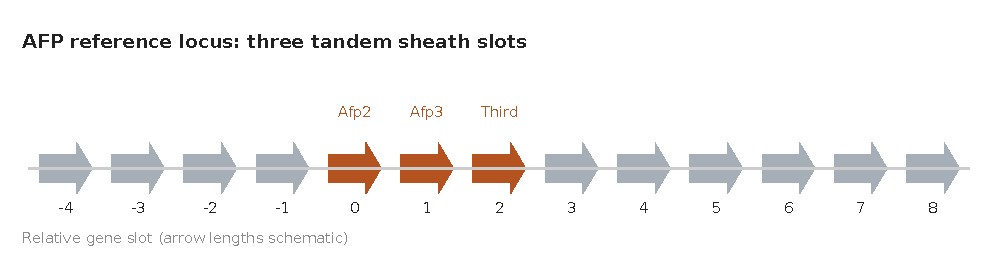
\includegraphics[width=\textwidth,height=0.14\textheight,keepaspectratio]{figures/FigureS3a.pdf}\par\smallskip
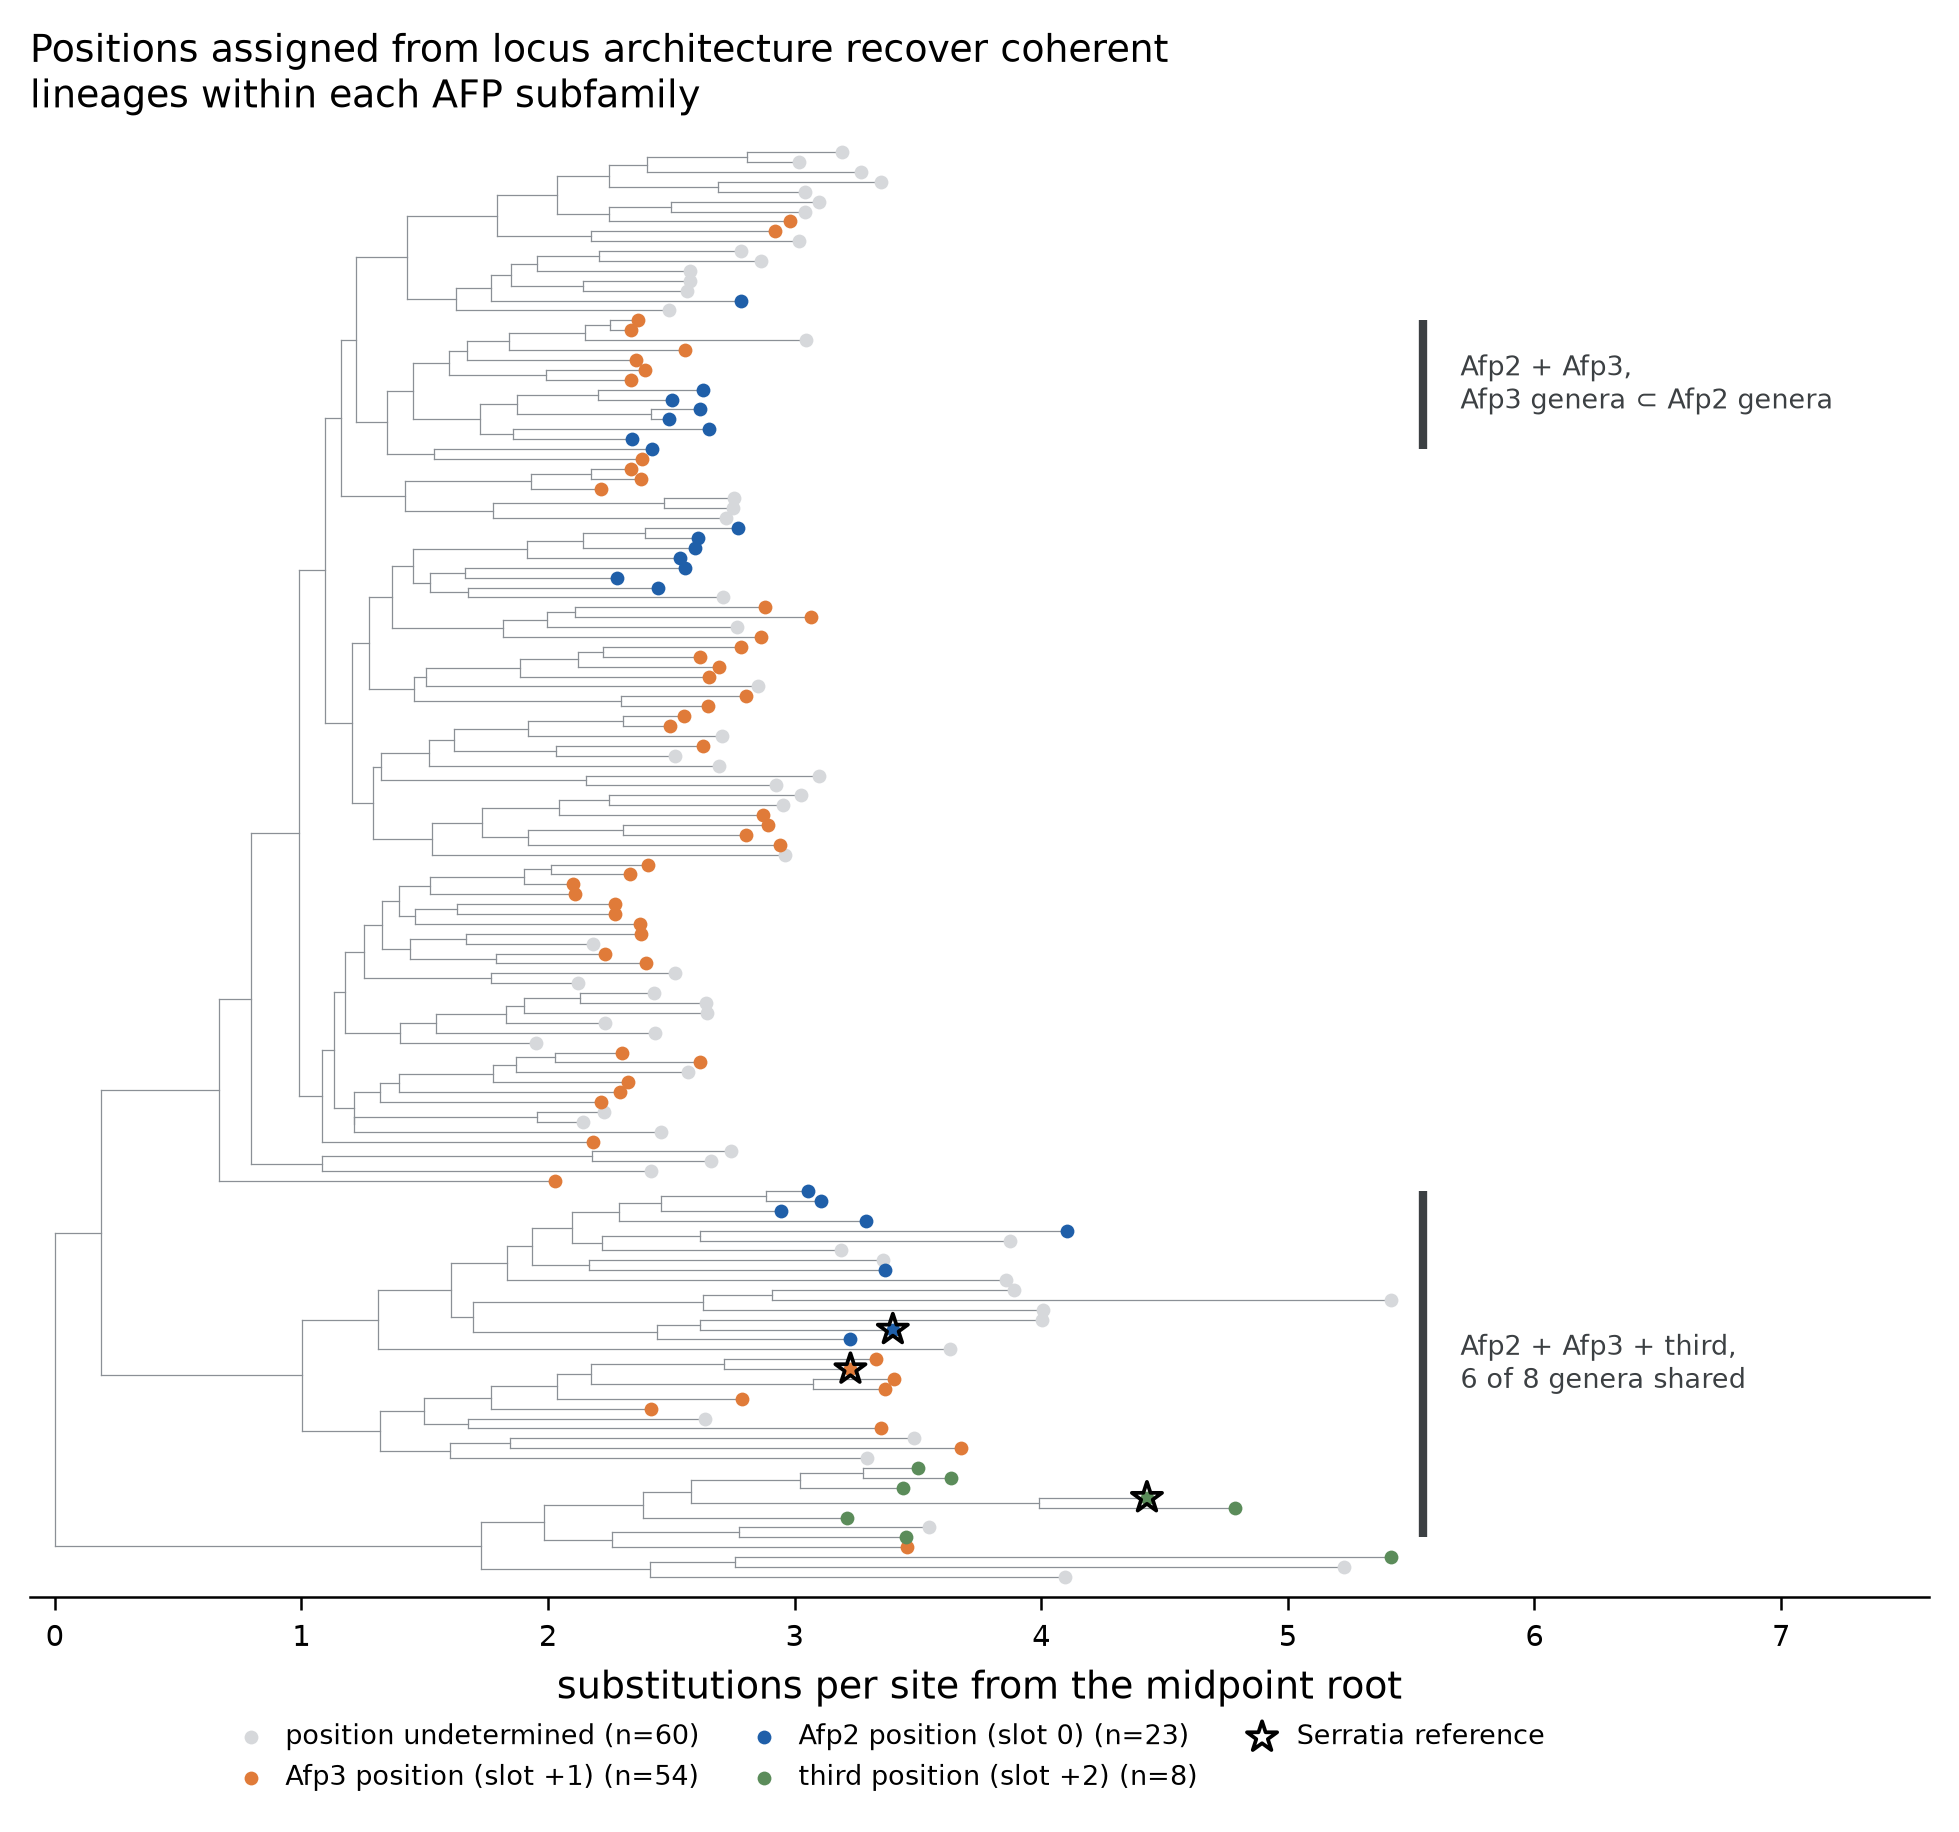
\includegraphics[width=\textwidth,height=0.58\textheight,keepaspectratio]{figures/FigureS3b.png}\par\smallskip
\caption{AFP locus architecture and phylogenetic assignment. (a) Reference-neighbourhood gene order from the saved annotation, oriented relative to the sheath. Arrows show CDS orientation and relative order, not nucleotide lengths; sheath slots 0--2 are highlighted. (b) Existing 145-tip joint FastTree diagnostic phylogeny with positional classes and reference tips. It is distinct from the final protein-specific IQ-TREE rate topologies.}
\label{fig:supp3}
\end{figure}

\begin{figure}[p]
\centering
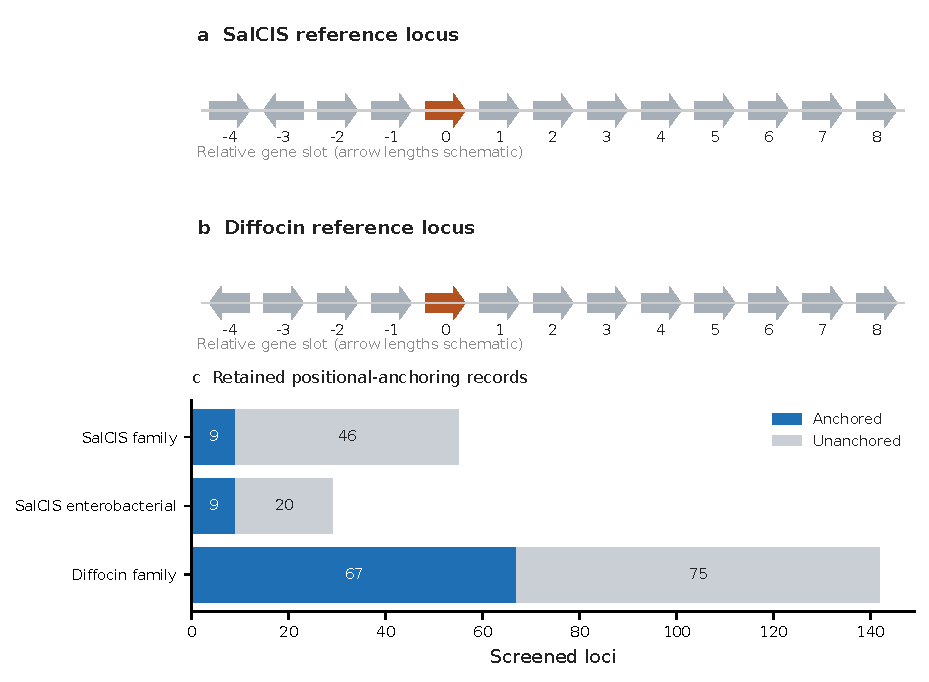
\includegraphics[width=\textwidth,height=0.70\textheight,keepaspectratio]{figures/FigureS4.pdf}\par\smallskip
\caption{SalCIS and diffocin positional evidence. Reference gene order and counts of anchored/unanchored loci are drawn from saved annotation and locus tables. SalCIS shows family-wide and restricted enterobacterial assessments; diffocin shows the family-wide assessment. These screening-stage counts do not equal final rate-dataset sizes. Arrow lengths are schematic. Diffocin's local single-sheath pattern does not rule out multiple loci per replicon.}
\label{fig:supp4}
\end{figure}

\begin{figure}[p]
\centering
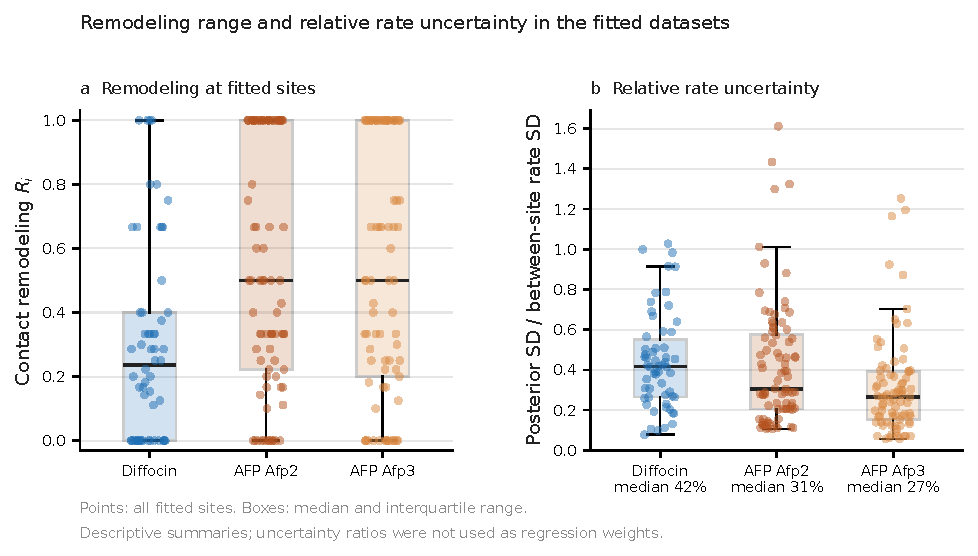
\includegraphics[width=\textwidth,height=0.65\textheight,keepaspectratio]{figures/FigureS5.pdf}\par\smallskip
\caption{Descriptive remodeling range and relative posterior rate uncertainty at the primary fitted sites. Posterior SD is divided by the sample SD of point-estimated rates within each protein. Points and boxes summarize saved site tables. This is an existing descriptive diagnostic, not a new power calculation, uncertainty-propagation model or regression weighting scheme.}
\label{fig:supp5}
\end{figure}
